Machine learning requires that the data possesses sufficient characteristics to approximate the sample population from which it was extracted. Therefore, we examine the data in attempt to remove outliers and determine if the data is sufficient for classification. In addition, in a particular case study, certain tumors have been shown to be heterogeneous \cite{friedmann2014glioblastoma}, this can be problematic for a classifier as heterogeneous samples lack in shared characteristics. 

In this chapter, we examine the data available to the project. In particular we investigate how the Raman spectra have been prepared, as their processing is essential for analysis. We undergo several steops as follows. First, we describe the mathematical representation of the samples. Since the number of samples is rather small for learning, we explain how each sample may be separated into individual spectra; this separation yields a drastic increase in the number of available training examples. Second, we explain how to balance the data; an unbalanced dataset would likely introduce bias during learning, rendering the models desired predictive capabilities uncertain. We achieve this by duplicating samples belonging to underrepresented categories in the dataset. Furthermore, this balancing is performed to maintain majority and minority categories, thus retaining some distributional information from the original dataset. The main goal of our analysis is to analyze the data using different methodologies for detecting spectra which has been altered due to non-tumor material affecting the spectra (henceforth called outliers). As a starting point for our analysis, we have defined the frequency criterion. The criterion is used to separate tumor spectra from outliers in each sample. The outliers captured by this criterion is compared to outliers detected by other outlier detection techniques such as the Standard Deviation Test (SDT) and the Interquartile Range Method (IRM). The unsupervised machine learning methods \textit{K-means} clustering and hierarchical clustering are also used in attempt to detect outliers in each sample. The results from each method are then compared to select the one which best separates outliers from the tumor spectra, after which the data is curated by that method.

Another point of interest in this project is the identification of representative frequencies within the spectra. Each spectra belongs to a tumor which can be categorized by six different categories. Our hypothesis states that certain frequencies should be sufficient in determining which category the tumor belongs to. Feature selection is used for this purpose, representing each frequency within the spectra as distinct features. However, in order to extract such features reliably, the data must be devoid of outliers. Should outliers exist within the dataset, the features given by the methods used will be influenced by the outliers. To prepare for this, the data is plotted for visual inspection. It is confirmed by the data provider that the majority of samples include outliers. These outliers are influenced by a variety of other materials found on the tissues surface, e.g., spectra of blood drops, plastic which may be reflected form underneath thin tissue or necrotic tissue, which is shown to affect the spectral signal. Using the extracted features, a model can be trained on the data faster which can be essential, as many machine learning methods require a significant amount of computing resources and data. The features are extracted before and again after the removal of problematic spectra. This is done to compare the impact of the outliers in feature selection. We expect the features yielded vary significantly for different subsets of the available data. Feature selection is not a good strategy for machine learning in this particular case if the features extracted from different subsets vary tremendously. If different subsets of the data are best represented by different features, a model can accidentally be trained to only consider one set of features which will yield poor performance on unseen data.


\section{Data Representation}
The data consists of the Raman spectra extracted from the tissue of glioma tumors from 45 patients. Multiple samples of tissue were extracted from the same patient in some cases, yielding several samples for the respective patient. To maintain separation among the patients, the samples are sorted by their respective patient of origin. This is necessary due to the heterogeneity of each tumor. The data will be separated into three separate datasets. These sets are referred to as the training set, the validation set and the test set. Due to the expected heterogeneity, all datasets will consist of unique patients to avoid scenarios in which the model overfits to a patients tumor sample. This structure also allows for easier handling of the number of patients in each sample category, allowing for analysis on each category separately from the others.

There is also large variation with regard to the sample shape within the data. Each sample is a 3-dimensional array of shape $(w, h, 1738)$ where $w$ and $h$ are the width and height of the sample, respectively. This formalization is necessary, as width and height have non-zero variance among different samples. The shape is a result of how the tissue was scanned. In each case the tissue was placed inside the Raman spectrometer and scanned successively from side to side. This makes it possible to display each sample as an image, by substituting the third dimension (denoted above by $1738$) with a color value denoted by which category the spectra belongs to. The number $1738$ is constant through all samples and represents the length of a modified Raman spectra. The spectra has been modified by the data provider; the data consist of spectra resulting of a linear mapping from the extracted spectra. This is done to omit unnecessary frequencies and allow focus on parts of the spectra which we believe are sufficient for this project. Furthermore, each element inside these arrays is a real number without clear bounds. The largest absolute element found within the complete dataset is $79427.0625$. Some values are negative, which is confirmed by the data provider to have significance for the project's purpose. The project aims to prepare these spectra for use in machine learning methods. Predictions should be performed on individual spectra extracted form the dataset. We choose this strategy since each spectrum is independent of all other surrounding spectra, ideally sharing in some characteristics from the other spectra belonging to the LGm category we wish to predict, i.e., one spectrum should describe which LGm category the sample belongs to. There are six distinct LGm categories as defined by Ceccarelli et al. \cite{cellsubsets}, denoted LGm1 - 6. The model will take as input one vector of shape $(1, 1738)$ and produce one vector of shape $(1, 6)$. This strategy is inspired by Liu et al. \cite{liu2017deep}, who managed to get satisfactory performance by training a model on raw spectra i.e. spectra without preprocessing or outlier removal. Restructuring of the data to represent all samples as a list of spectra rather than 3-dimensional matrices yields a dataset with more than $300,000$ datapoints, which is a sufficiently large dataset for machine learning.

Initially, we choose to examine each sample by plotting the spectral lines in a plot. This allows us to examine the general shape and visually deduce if any common patterns are present in the samples and identify problematic samples. As expected from analogue measurements, significant amounts of noise are present in each plot. Despite this, many spectra share in some general characteristics with a few spikes appearing on an mostly flat spectral line. An example of the plots created for this examination be seen in Figure \ref{fig:spectrum}.

\begin{figure}[h]

    \centering
    \subfloat[\centering Spectra from patient HF-1293. The rest of the samples available share in this pattern with some deviations]{{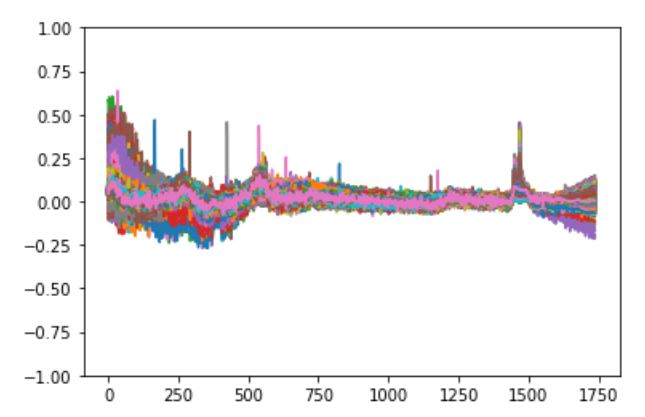
\includegraphics[width=5cm]{images/1293graph.JPG} }}
    \qquad
    \subfloat[\centering Spectra from patient HF-1887. The frequencies tilt towards the upper part of the plot. The example is decidedly removed from the analysis.]{{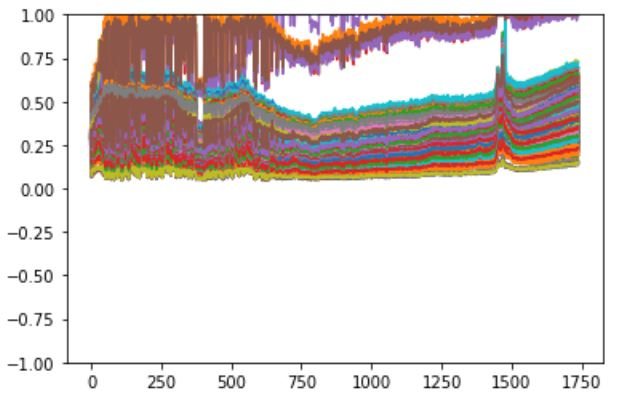
\includegraphics[width=5cm]{images/1887graph.JPG} }}%
    \caption{Examples of samples drawn from the data, HF-1293 display a common pattern across all samples, HF-1887 is removed due to the skewed baseline. The range of the values are normalized between -1 and 1 to easier display the spectra.
    \label{fig:spectrum}}%
\end{figure}

In Figure \ref{fig:spectrum} is shown two collections of spectra, the spectra belonging to sample HF-1293 are shown in Figure \ref{fig:spectrum} (a) and spectra from sample HF-1887 are shown in \ref{fig:spectrum} (b). The spectra form HF-1293 follow a general pattern visible in the vast majority of sample plots.
Sample HF-1887 is an example of one sample which we deem too sporadic for this project, we remove it due to the skewed baseline of all spectra in the sample after confiding with the data provider, who agrees with our decision. After visual examination, we can confirm that some characteristics are present, but they are not sufficiently different among the different LGm categories to be classified by a human being in this case. Machine learning is needed to detect precise differences    among the samples.

Another reason to remove samples are due to their size. The analysis we aim to perform requires considerable computational power and memory space. Many of the samples available have a manageable size, as they consist of approximately $3600$ spectra i.e. width and height are approximately $60$ and $60$ respectively. In case the samples are too big for use we may simply extract a random sub sample from the larger sample and analyze those. But applying that method at this stage would potentially ruin the form of the samples which is used to evaluate the outlier detection methods in a later section. Fortunately only one sample suffers from this problem. Sample HF-3097, shown in Figure \ref{fig:HF3097}, shows a concerning number of spikes in contrast to the other samples and is the only sample which require considerable memory space (the number of spectra exceed $40000$).

\begin{figure}[H]

    \centering
{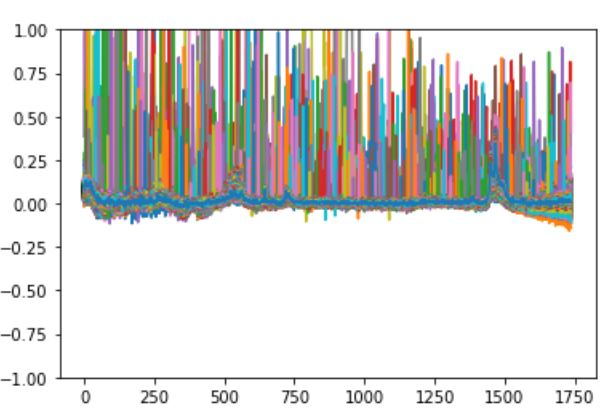
\includegraphics[width=5cm]{images/HF_3097.JPG} }
\caption{Sample HF-3097 from LGm2, the spectra spikes are extremely sporadic. The range of the values are normalized between -1 and 1 to easier display the spectra.\label{fig:HF3097}}%

\end{figure}

The values inside the spectra are also considerably bigger than the values found in the other samples. The methods SDT and IQM require statistical constants be extracted on the entire dataset, including this sample would affect the standard deviation and the mean of the frequencies tremendously (even if the constants were evaluated within the scope of the sample itself). K-means clustering is also a unsupervised machine learning model which can be trained on data before predictions are performed on unseen data. Since the aim is to use the training set  for training the model, inclusion of the sample would affect the performance considerably. If the sample is put in the test set for testing, the noise in the signals would affect predictions considerably, which would affect testing accuracy due to what appears to be noise in the frequencies. To avoid these statistical issues and to reduce the computational requirements, the sample is discarded following the data providers approval.


\section{Balancing the Data}
The model will, as a consequence of the learning algorithm, become biased towards certain predictions if presented with frequent examples of a particular category. As the model encounters frequent training examples, the connections which produce such predictions will strengthen. Over exposure to examples of a certain category will force the model to associate features with that category, redirecting focus from categories for which that feature could be significant. This is why it is important to train models on balanced data. Having a balanced dataset means the number of examples in each category are uniform in the entire training set. Training on a balanced dataset also avoids bias towards data distribution, where certain categories may be predicted more frequently than others simply because the distribution was used in training. The initial data suffers heavily from this problem. Training on the data would result in a model which produces frequent predictions for the majority category (the category which has the most spectra) and perform inconsistently for the other categories. The data distribution is shown in Table \ref{table:1}.

\begin{table}[htb]
\centering
 \begin{tabular}{||c c c c c c c||} 
 \hline
 Category & LGm1 & LGm2 & LGm3 & LGm4 & LGm5 & LGm6 \\ [0.5ex] 
 \hline\hline
 \# Of samples & 5& 11 & 4 & 10 & 11 & 4 \\ 
 \hline
 \# Of spectra & 37319 & 71846 & 31931 & 50660 & 62256 & 20176 \\
 \hline
 Percentage & 14\%& 26\% & 12\% & 18\% & 23\% & 7\% \\
 \hline

\end{tabular}
\caption{The distribution of data in the initial dataset after removing the problematic samples.}
\label{table:1}
\end{table}

Table \ref{table:1} shows the categorical separation in the data, the header row shows the labels of each category. The first row shows the number of samples belonging to each category, these are the tumors which will be analyzed. The second row displays the total number of spectra across each category; these must be considered for balancing. Note the equal amount of samples in LGm3 and LGm6, but the difference in number of spectra within them. This is due to the varying size of all samples drawn from the tumors. Some samples share the same size, however the important fact is that the samples lack a uniform shape, which must be considered during the analysis. The last row shows the percentage each category makes of the entire dataset. Initially LGm2 is the majority category while LGm6 is the minority category, consisting of only $7$\% of the entire dataset.

Before the data is balanced, the testing data is selected and separated from the rest. This is done by separating at least one patient and all their samples from the rest of the data. This way, we ensure the possibility to test if the model develops bias towards the patients in training and if the patient samples are heterogeneous with respect to the other samples of the same category. Samples are chosen with the criterion that approximately $30\%$ of each category is represented in the test set. Balancing the categories which contain less elements by a factor larger than or equal to two compared to the majority category (LGm2) is done by repeating the spectrum in each sample by that factor. This methods does not perfectly balance the data to have a uniform distribution of categories, but it does make the underrepresented category frequent enough to circumvent the issue of unbalanced datasets. The multipliers for each categories are chosen so as to retain the majority category i.e. LGm2 will remain the majority category after balancing is done. There is also a need for the validation set, the validation will be used to monitor the models performance on unseen data during training. The samples for this set are chosen such that one sample from each category is allocated to the set. The separation of the entire dataset into three distinct sets is arbitrary and so can be performed automatically. However, we choose to perform this separation manually to maintain consistency in this analysis. The resulting separation is shown here as it is the training set from which the features are extracted in this project. We discover that the results will differ slightly depending on which samples are chosen for which set. The distribution of all datasets are shown in Table \ref{table:2}.

\begin{table}[H]
\centering
 \begin{tabular}{||c c c c c c c||} 
 \hline
 Category & LGm1 & LGm2 & LGm3 & LGm4 & LGm5 & LGm6 \\ [0.5ex] 
 \hline\hline
 \# Training & 17689 & 47602 & 37557 & 30180 & 33396 & 9376 \\
 \hline 
 \# Validation & 3600 & 4096 & 3600 & 4096 & 4096 & 3600 \\
 \hline
 \# Test & 14945 & 20140 & 11296 & 16384 & 24764 & 7200 \\
 \hline

\end{tabular}
\caption{Distribution of the three datasets}
\label{table:2}
\end{table}

Table \ref{table:2} shows the distribution of the different datasets used in this project. The training set is then balanced exclusively. This is not required in the test set or the validation set, since they will have no direct effect on how the model is developed through training. It is also important that the validation and test sets are not uniform, since it will prove whether the model can generalize to different prediction distributions. The training set is balanced by replicating each spectra in every patient of the categories which are under-represented. The number of sample replications per category can be computed by the following method. Let $m$ be the LGm category which contains the majority of spectra in the set and $|LGm_n|$ be the number of spectra in LGm category $n$. The number of replications for each category can then be computed by $\lfloor \frac{|LGm_m|}{|LGm_n|} \rfloor$. The distribution of the training set after applying the replication method is shown in Table \ref{table:3}.

\begin{table}[htb]
\centering
 \begin{tabular}{||c c c c c c c||} 
 \hline
 Category & LGm1 & LGm2 & LGm3 & LGm4 & LGm5 & LGm6 \\ [0.5ex] 
 \hline\hline
 \# Training & 35378 & 47602 & 37557 & 30180 & 33396 & 46880 \\
 \hline 
 Percentage & 15.32 & 20.6 & 16.26 & 13.07 & 14.46 & 20.29 \\
 \hline 

\end{tabular}
\caption{Distribution of the testing data following balancing}
\label{table:3}
\end{table}

As is shown by the last row in Table \ref{table:3}, the data does not have a uniform distribution as LGm2 is still significantly larger than LGm4. However, the important thing is that the distribution is better balanced relative to the original distribution. The biggest difference between the categories is by approximately seven percent. We assume this distribution is good enough and proceed to the next step of the analysis.


\section{Feature Selection and Visual Analysis}

Following the balancing, the first step in the analysis is to find the frequencies which best describe the data with respect to the different categories. Each number in the spectra is a frequency at which the scattered light is gathered. This light is expected to be sufficient for predicting the categories of the tumor-tissue. We assume that, to sufficiently categorize the spectra into the categories, only certain frequencies are required. For this reason, the most significant features are extracted with SelectKBestfeatures \cite{scikit} which is given the f-classif method for ranking the features in order of their significance. Following this step, we may pick any arbitrary number of features by extracting them in the order given by f-classif. The $70$ best features are extracted from the training set in which there are outliers present still. The features are displayed in Appendix \ref{appendix:features0}. The extracted features show that regions of interest do exist on the spectra. This can be seen by the integers which have a successive difference of one, suggesting that the region of interest exist somewhere in specific parts of the spectra. It is worth noting here that the features selected might be correct provided the amount of outliers is sufficiently small to be ignored by the feature selection method. Due to this uncertainty, the data will be separated from the outliers and feature selection will be performed a second time at the end of this section.

All data is subject to this analysis as all samples must be curated before the model can be trained. In the methods where statistical constants must be calculated, the training data is used, this avoids bias towards the other datasets whose primary purpose is to evaluate the model. The goal of the analysis is to find a uniform criterion which each spectrum must fulfill to be considered \textit{clean}. Spectra which fail to satisfy this criterion will be discarded form the project entirely. In this section the methods of analysis used are described and their results examined. The section begins by examining the frequency criterion, which is a confirmed criterion all spectra must satisfy to be considered "clean". This criterion was provided by the data provider. SDT and IRM are compared to the frequency criterion for validation, these are deterministic methods that rely solely on the values found within the data and are commonly used to detect outliers in data. \textit{K-means} clustering and Hierarchical clustering are then performed on the data in attempt to capture potentially complex patterns within the data. These methods are specifically designed to allow for grouping of data based on the similarities between data points within the dataset. The section ends by selecting the method which best detect outliers, this method is then added to the preprocessing stage i.e. following this project, all samples must be curated using this method before they can be used by the machine learning model. 

\subsection{The frequency criterion}

The frequency criterion is a criterion specified by Adrian Lita for separating outlier spectra from tumor spectra. The criterion states that, should any value of frequencies between $1463$ and $1473$ of any spectrum be below $5000$, then that spectrum is defined to be and outlier. Given that this criterion is defined by the provider, together with the lack of knowledge regarding where outliers may be positioned on the samples, we choose this criterion as the starting point of this analysis. The extracted features in Appendix \ref{appendix:features0} include parts of the range on which the criterion is based, which is promising. The range being present in the extracted features can also mean that the outliers work to influence the relationship between the spectra and the categories we want to predict. In which case the removal of the outliers are essential for building an unbiased model. We examine the results of the criterion to gain insight into where these outliers are positioned. The criterion is confirmed to miss some outliers and so it mainly functions as an initial approximation of the areas where outliers are present. An example of this is in sample HF-2849 of LGm3 shown in Figure \ref{fig:HF2849_1}.

\begin{figure}[H]

    \centering
{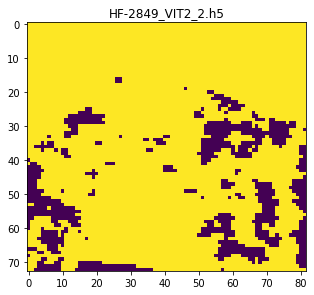
\includegraphics[width=4cm]{images/AdriansCriterion/LGm-3/HF-2849_VIT2_2.h5_5.png} }
\caption{Sample HF-2849 from LGm3. The sample is confirmed to have necrotic tissue present in the upper part.\label{fig:HF2849_1}}%

\end{figure}

The criterion is satisfactory for capturing areas in the lower parts of the sample. However, the upper part of the sample is guaranteed to have spectra from necrotic tissue which is unreliable for describing the LGm Category of the tissue. It appears the criterion is well suited for detecting liquid material on the tissue, since many samples show smaller spots of interest and fail to completely capture larger areas of outliers. This is evident in Figure \ref{fig:HF2849_1}, as multiple small spots are detected. This is one of several examples for how the criterion fails to detect all outliers reliably, but in the majority of the samples, the outliers are detected sufficiently well. One such case can be seen in sample HF-868 displayed in Figure \ref{fig:ADHF868}.

\begin{figure}[H]

    \centering
{\includegraphics[width=3cm]{images/AdriansCriterion/LGm-1/HF-868_1_2.h5_0.png} }
\caption{Sample HF-868 from LGm1. The areas detected are confirmed outliers.\label{fig:ADHF868}}%

\end{figure}

According to the data provider, the outliers present in HF-868 are sufficiently captured by the frequency criterion. The outliers form as small, sporadic areas on the surface of the tissue. This shape is what the outliers are expected to have in the samples which are known to include them. However, since the frequency criterion fails to capture outliers in certain samples (possibly due to the material information of those outliers), we explore changes made to the criterion e.g. making the interval greater (checking frequencies ranging from 1458 to 1478) and checking for frequencies which are below $20000$ within the interval the criterion concerns. The results vary greatly from the original criterion. Though some of the spectra originally ignored by the criterion now become visible, not all regions are sufficiently captured. This indicates the necessity to use other parts of the spectra which appear to be relevant for outliers. The spectra are too big for further manual inspection, which greatly motivates the application of machine learning methods. The frequency criterion will, however, serve as a ground truth in this analysis. Going forward in this section we aim to evaluate all following methods by comparing them to the results of the frequency criterion. Examples which best reflect the methods performance in outlier detection will be displayed for comparison with this criterion. This way, we have some knowledge about where outliers are detected. While the criterion is insufficient in detecting all  outliers (as demonstrated in this subsection), the general patterns discovered here must be present in the results yielded by the other methods. If the method under analysis fails to produce results corresponding to the frequency criterion, we opt to disregard that method. The desired method optimally produces similar results as the frequency criterion and finds more areas on the samples where we know outliers are present. Ideally, the methods also aid in discovering new outliers.

\subsection{The standard deviation test}

We investigate the data using the standard deviation test is a test by which the data is centered around the mean and given a standard deviation of one. With this setup, outliers are defined as points which are separated from the mean by three standard deviations or more. We measure the mean and standard deviation on each frequency from the unbalanced training set; we ignore the balancing to avoid changes to the mean and standard deviation which the balancing helps produce. The values are then used to standardize the spectra belonging to each tumor. A spectrum is deemed to be an outlier if the number of frequencies in that spectrum exceed an arbitrary value. We approximated the value by performing the test once while monitoring the average number of frequencies which lie three or more standard deviations from the mean. In any given sample, each spectrum includes on average $111$ frequencies which fail the test. We specify that a spectrum fails the test if more than $111$ of its frequencies are three or more standard deviations away from the mean.

Using this test, many small areas are detected in each sample, it suggests there is something present in those places, but they do not possess a clear shape by which we can decide whether to discard them or not. An example of such a sample is shown in Figure \ref{fig:stdHF448}.

\begin{figure}[H]

    \centering
    \subfloat[\centering The result of SDT for sample HF-448, Several points are labeled as outliers]{{\includegraphics[width=4cm]{images/STDtest/LGm-1/HF-448_V5B_1.h5_3.png} }}
    \qquad
    \subfloat[\centering The frequency criterion outliers for HF-448]{{\includegraphics[width=4cm]{images/AdriansCriterion/LGm-1/HF-448_V5B_1.h5_3.png} }}%
    \caption{A comparison between the SDT and the frequency criterion for sample HF-448.
\label{fig:stdHF448}}%
\end{figure}

SDT does not produce results similar to the frequency criterion, some spectra do correspond among the results, but the amount of outliers falsely labeled as outliers by SDT is troublesome. Roughly $50\%$ of the samples in the entire dataset yield similar results with SDT. The method would as a result of this, discard too much from most samples, depraving the dataset of a great number of tumor spectra. Some areas are formed around the individual spectra, suggesting the presence of an unknown material, but the sporadic points in the surrounding area make it unclear where that material begins and ends. Furthermore, we must develop a criterion for which points to discard. Such a criterion would need to distinguish between sporadic points which are miss-classified and areas of real outliers. However, within some samples there are areas of outliers correctly labeled, but those areas are not sufficiently defined. One sample with this result is shown in Figure \ref{fig:stdHF868}.

\begin{figure}[H]
    \centering
    \subfloat[\centering The result of SDT for sample HF-868]{{\includegraphics[width=4cm]{images/STDtest/LGm-1/HF-868_1_2.h5_0.png} }}
    \qquad
    \subfloat[\centering The frequency criterion outliers for HF-868]{{\includegraphics[width=4cm]{images/AdriansCriterion/LGm-1/HF-868_1_2.h5_0.png} }}%
    \caption{A comparison between the SDT and the frequency criterion for sample HF-868. Many spectra correspond to the frequency criterion.
\label{fig:stdHF868}}%
\end{figure}

Sample HF-868 is less sporadic compared to HF-448, the outliers are instead formed around common points of interest which strongly suggests outliers are present in that area. The lack of definition in each area however, is not sufficient. The outliers must form concrete shapes with clear definition. The sample suggests outliers are present in the different areas, but all points are not present to make the shapes as defined as they are by the frequency criterion. 
The sporadic results show that this method is insufficient to detect the majority of outliers in all samples. It must be noted that despite this underwhelming result, some outliers are detected, suggesting further changes to the method could yield better results, though greedy application is not going to work for all samples. Throughout all the six LGm categories, the method yields the best results for LGm6 where it shares many patterns with the patterns produced by the frequency criterion. Another example of the methods promise is in sample HF-2852 of LGm3 shown in Figure \ref{fig:stdHF2852}.

\begin{figure}[H]
    \centering
    \subfloat[\centering The result of SDT for sample HF-2852]{{\includegraphics[width=4cm]{images/STDtest/LGm-3/HF-2852_VIT_2_2.h5_6.png} }}
    \qquad
    \subfloat[\centering The frequency criterion outliers for HF-2852]{{\includegraphics[width=4cm]{images/AdriansCriterion/LGm-3/HF-2852_VIT_2_2.h5_6.png} }}%
    \caption{A comparison between the SDT and the frequency criterion for sample HF-2852.
\label{fig:stdHF2852}}%
\end{figure}


Sample HF-2852 has a large area in the upper part which consists of necrotic tissue. The spectra of that tissue differs from other spectra sufficiently well, allowing the method to distinguish between tumor and non-tumor with considerable accuracy. This is due to the amount of otherwise healthy tissue present in the sample. The methods inability to capture all outliers is also present despite this, as it allows several smaller spots in the area of the necrotic tissue to be classified as healthy tumor tissue. The area at the bottom of the sample is filled with outliers according to the frequency criterion. These results suggests that the method is best used in detecting necrotic tissue, but not in context of detecting other kinds of outliers.

\subsection{The Interquartile range method}

Similar to SDT, IRM is a purely statistical analysis method, detecting outliers in terms of which percentile the spectra belong to. The 25th and 75th percentiles are calculated on each frequency for the entire training set. Like SDT, this method yields a varying amount of outliers for each sample. We instead define the allowed number of outlier frequencies within one spectra to be equal to the average number of outlier frequencies within the analyzed sample. Many regions are better represented by IRM, showing well defined areas where outliers are clearly present. The amount of individual spots are less frequent which shows promise in the method, as e.g. blood is expected to cover a larger area if present. The improvement from the standard deviation test is seen in Figure \ref{fig:iqrHF448}.

\begin{figure}[H]

    \centering
    \subfloat[\centering The result of the interquartile range for HF-448, Several well defined areas are separated form the majority of spectra]{{\includegraphics[width=4cm]{images/IQR/LGm-1/HF-448_V5B_1.h5_3.png} }}
    \qquad
    \subfloat[\centering The standard deviation test for sample HF-448]{{\includegraphics[width=4cm]{images/AdriansCriterion/LGm-1/HF-448_V5B_1.h5_3.png} }}%
    \caption{A comparison between IRM and the frequency criterion for sample HF-448.
\label{fig:iqrHF448}}%
\end{figure}

SDT failed to separate outliers adequately in sample HF-448 while IRM is better suited to detect the outliers in this sample. The upper part of the sample has a well defined line where the sample is presumably cut, meaning the plastic underneath the tissue might be visible. We also note that many outliers detected by IRM also appear to be captured by SDT. While the areas are hard to distinguish among all sporadic spots, the larger spots in Figure \ref{fig:iqrHF448} (a) seem to have some trace in Figure \ref{fig:stdHF448}. The correspondence with the frequency criterion in Figure \ref{fig:iqrHF448} (b) further shows the methods capability in contrast to SDT as the method seem to possess greater ability in defining the areas where outliers are present. There are still some spots appearing randomly around the sample surface which would ideally be ignored, but while we have some confirmation on where outliers are present in certain samples, we do not know exactly where the outliers are. The individual points being labeled as outliers suggests the method struggles with the same issue SDT suffers from. Though it appears to be less severe in all samples belonging to LGm1, there are still a considerable amount of spots through all samples within the category. Especially LGm4 have samples for which both methods perform poorly, with a considerable amount of sporadic spots appearing in some samples when applying IRM and a significant lack of spots when applying SDT i.e. None of the methods works sufficiently well to detect the outliers. It should be noted that both methods detect outliers in areas which the frequency criterion also produces. But the areas are not corresponding well in either method. This issue is apparent in sample HF-2802 of LGm4, shown in Figure \ref{fig:HF2802comp}.

\begin{figure}[h]

    \centering
    \subfloat[\centering The result of the interquartile range for HF-2802, some larger areas are detected with sporadic spots around the entire spectra.]{{\includegraphics[width=4cm]{images/IQR/LGm-4/HF-2802_V3T_1.h5_11.png} }}
    \qquad
    \subfloat[\centering The result of the standard deviation test for HF-2802. Few outliers are detected]{{\includegraphics[width=4cm]{images/STDtest/LGm-4/HF-2802_V3T_1.h5_11.png} }}%
    \caption{A comparison between the interquartile range and the standard deviation test for sample HF-2802. In comparison, the interquartile range locates better defined areas than the standard deviation test, but many sporadic spots are present.
\label{fig:HF2802comp}}%
\end{figure}
 

In Figure \ref{fig:HF2802comp}, the results of IRM and SDT are compared on sample HF-2802. Both methods yield poor separation between the outliers and tumor spectra. IRM is capable of detecting a large mass of some material on the sample, however, many sporadic spots appear around it, the majority of these spots are tumor spectra which would be discarded by the method. In stark contrast, SDT struggles to detect anything in the sample, only yielding small spots in the larger areas found with IRM.
Fewer samples suffer from the stochastic results present in SDT, however all samples are not strictly improvements from SDT. One such example is sample HF-1010 belonging to LGm2, shown in Figure \ref{fig:HF1010comp}.

\begin{figure}[h]

    \centering
    \subfloat[\centering The result of the interquartile range for HF-1010]{{\includegraphics[width=3cm]{images/IQR/LGm-2/HF-1010_V1T_1.h5_8.png} }}
    \qquad
    \subfloat[\centering The result of the standard deviation test for HF-1010.]{{\includegraphics[width=3cm]{images/STDtest/LGm-2/HF-1010_V1T_1.h5_8.png} }}%
    \caption{A comparison between the interquartile range and the standard deviation test for sample HF-1010, LGm2.
\label{fig:HF1010comp}}%
\end{figure}

The comparison in Figure \ref{fig:HF1010comp} show one of few samples where IRM fails to sufficiently separate outliers from tumor spectra. A considerable number of spectra are falsely labeled as outliers, and those spectra seem to form many smaller areas without sporadic points in the surrounding area. In this rare case, SDT exhibits sufficient separation of the outliers, as the detected areas correspond well with the the position of known outliers found by the frequency criterion.

Few samples follow the same conclusion however, these varying results show clear signs that neither of the methods are suitable to perfectly rid each sample of outliers. We therefore dismiss them from the analysis, while keeping the results for comparison with the other methods. We continue the analysis by analyzing unsupervised machine learning methods for outlier detection.

\subsection{Hierarchical clustering}

The next method for outlier detection is hierarchical clustering, we choose to utilize the \textit{agglomerative} version of the algorithm. Due to the algorithms demanding time complexity and memory constraints, we analyze each sample separately to avoid memory errors. Each sample must be given one unique model which then divides the data into  the number of clusters specified. This means there will not be a universal model designed to separate all samples. We investigate the results of different distance metrics and choose \textit{Euclidean distance} as distance metric to measure distance among the clusters. This conclusion is due to the uncertainty in vector shape and angles on which Cosine similarity is dependent. The \textit{Manhattan distance} would be a better choice compared to \textit{Cosine similarity}; however, \textit{Euclidean distance} magnifies long distances, which should aid the algorithm in selecting clusters for \textit{agglomerative} merging. Next we examine the linkage criteria available. In each case, the algorithm is set to run multiple tests where it separates the data into different amounts of clusters. We choose to initialize five different models to compute between two and seven clusters respectively. Due to the deterministic nature of the algorithm, the results in one cluster will be present in the other clusters as the the number of clusters increases.

Single linkage merges clusters which posses points with minimal distance. Should the spectra within the samples be significantly "far apart" in the data, the criterion might start producing many unique clusters in a "chain". If the number of clusters are sufficiently small, the number of cluster separations will be few, and few spectra will be allocated to those clusters. This can result in few separations for some samples, which will render the method unusable for our purposes.

The criterion yields clusters which appear as individual points in the spectra and fail to detect areas where known outliers are present in the samples, suggesting the aforementioned flaw is present in this methodology. This is apparent as we see few cluster areas form in any of the initialized models, even if we allow the method to use more than two clusters. All different cluster models fail to separate the outliers and instead separate a small number of points. An example of this phenomenon is displayed in Figure \ref{fig:SL_HF868}.

\begin{figure}[H]

    \centering
{\includegraphics[width=15cm]{images/Single_linkage/LGm-1/HF-868_1_2.h5_0.png} }
\caption{Single linkage on sample HF-868 from LGm1, The test fails to detect any outlier areas. Leftmost image is the result of the model computing two clusters. The number of clusters increase towards the rightmost image.\label{fig:SL_HF868}}%

\end{figure}

The models fail to detect any areas where outliers are present, only yielding an insignificant number of outliers in the entire sample. Models computing more clusters also fail to find significant areas and smaller spots appear as the number of clusters increase. As the number of clusters increase, several of the outliers seem to belong to their own clusters, which is a sign of the clusters being computed in a "chain" as previously stated. Due to this unsatisfactory result, Single linkage will not be used as linkage criterion in this project.


Average linkage yields superior results compared to single linkage since some areas become more defined as we increase the number of clusters. Moreover, the criterion does not have a set number of clusters which is guaranteed to include all outliers for all samples. For certain samples the outliers are visible when forcing the algorithm to agglomerate to two clusters and others only show them once five or more clusters are allowed. It is possible to use the criterion for discarding the outliers if the majority cluster is preserved when computing seven clusters, while the rest of the spectra are discarded. However, this would not remove all outliers and some problematic samples in LGm3 would have the majority of outliers preserved. The improvement from Single linkage is made apparent in Figure \ref{fig:AL_HF868}.

\begin{figure}[H]

    \centering
{\includegraphics[width=15cm]{images/Average_linkage/LGm-1/HF-868_1_2.h5_0.png} }
\caption{Average linkage on sample HF-868 from LGm1, Leftmost image is the result of the model computing two clusters. The number of clusters increase towards the rightmost image.\label{fig:AL_HF868}}%

\end{figure}

The model computing two clusters is capable of producing separations where the outliers are present, though it still misses the bigger areas. As the number of clusters increases, the areas become more defined and capture more of the outliers. Despite this, all outliers are not detected even with seven cluster computed. One area should be captured in the lower left corner of the sample. However, only smaller clusters form around that area. Capturing it sufficiently would mean adding more clusters, but the number of clusters which best capture the outliers for all samples is variable in this case. It is a clear improvement over Single linkage, but the criterion is still not sufficient.

Complete linkage merges the clusters which posses elements with the smallest possible maximal distance between them. The method produces similar results as average linkage, few areas with outliers are detected when fewer clusters are permitted. However, some outliers are present when computing two or three clusters. Computing seven clusters allows the algorithm to detect outliers which are also detected by the frequency criterion. Though these results are not strictly improvements from average linkage, the criterion does manage to detect certain sports of outliers with fewer clusters than average linkage in certain samples. The result of complete linkage on sample HF-868 is seen in Figure \ref{fig:CL_HF868}.

\begin{figure}[H]

    \centering
{\includegraphics[width=13cm]{images/Complete_linkage/LGm-1/HF-868_1_2.h5_0.png} }
\caption{Complete linkage on sample HF-868 from LGm1. Leftmost image is the result of the model computing 2 clusters. The number of clusters increase towards the rightmost image.\label{fig:CL_HF868}}%

\end{figure}

As is evident in Figure \ref{fig:CL_HF868}, much like average linkage, complete linkage produces clearer areas as more clusters are computed. In HF-868, outliers are not detected earlier than average linkage, in fact, the outliers require more clusters to become apparent. A good approximation for the majority of samples appear to be the models computing seven clusters, if a few outliers are allowed to be included in the training phase of the model. The criterion's tendency to produce clusters earlier than average linkage is better displayed in Appendix \ref{appendix:HF1293Comparison}. Most samples display similar results; more outliers are detected overall with complete linkage in models computing two or three clusters than models using average linkage. Despite this, all five models fail to detect the outliers found by the frequency criterion. We therefore decide to disregard complete linkage for this project.

Ward linkage merges clusters which posses minimal variance between their respective elements and, as such, works well with \textit{Euclidean distance}. We do stress that the clusters are merged by measuring variance among cluster elements and there is no guarantee the outlier spectra should share in characteristics which would result in low inter-cluster variance. Despite this lack of guarantee, the clusters form at the precise location of outliers detected by the frequency criterion. Allowing seven clusters produce a near picture perfect image of the biological tissue from which the spectra were measured. These results show that the algorithm is capable of organizing the spectra according to their visual information which aid us in understanding shape and state of the samples. The criterion works considerably well for outlier detection when compared to the other criteria analyzed thus far. It appears to be capable of detecting well defined outlier areas, the individual points which appear around those areas appear to form smaller groups which could very well be individual droplets of the same outlier material detected in the larger areas. The promising performance of ward linkage is well represented in Figure \ref{fig:WL_HF868}.

\begin{figure}[H]

    \centering
{\includegraphics[width=15cm]{images/Ward_linkage/LGm-1/HF-868_1_2.h5_0.png} }
\caption{Ward linkage on sample HF-868 from LGm1. Leftmost image is the result of the model computing 2 clusters. The number of clusters increase towards the rightmost image.\label{fig:WL_HF868}}%

\end{figure}

The outliers identified correspond well with the frequency criterion, and as the number of clusters increase, the surface of the tissue starts to become visible by the different clusters. The model computing two clusters have near perfect resemblance with the frequency criterion. The models computing three and four clusters appear to perform subdivisions of the outlier cluster found in the model computing two clusters. This results tells us that the outliers appear to have significant differences from tumor spectra, which is a great result. We should expect similar results in samples which contain a great number of outliers. Once five clusters are allowed, spectra from healthy tissue starts to become apparent. These results appear to occur in the majority of samples.

The issue is finding a uniform criterion on which we can discard the outliers. We seek to define that criterion in terms of which clusters to discard from the samples following their analysis. Removing every cluster except for the majority cluster in the case where seven clusters have been formed would remove legitimate spectra which are suitable for training a model from all samples. In fact, there is no optimal choice in this case, as certain samples have their outliers sufficiently captured in a setup allowing for two clusters, while others show their outliers in arbitrary numbers of clusters. Furthermore, selecting clusters which contain close to $50\%$ of the spectra would be undesirable in context of maintaining a sizable dataset. By visual inspection, we deem the optimal number of clusters to be three, since many outliers are present in this choice, though the problem is not completely remedied. In some samples, ward linkage separates areas not outlined by the frequency criterion when two clusters are computed. The outliers are instead detected when computing more clusters. This complicates the process of finding a uniform criterion, but the number of outliers which are be missed by our current paradigm is considerably small. In particular, sample HF-2485 suffers from this problem, the cluster results are shown in Figure \ref{fig:hf_2485}.

\begin{figure}[h]

    \centering
{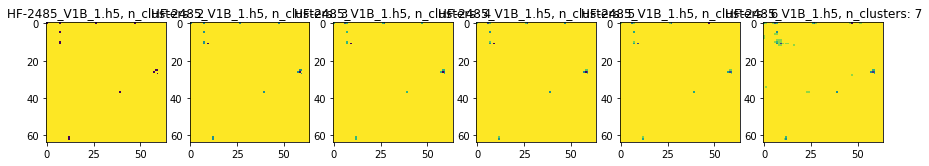
\includegraphics[width=15cm]{images/Ward_linkage/LGm-5/HF-2485_V1B_1.h5_9.png} }
\caption{Sample HF-2485 from LGm5, clustered by Hierarchical clustering using ward linkage. From left to right, is shown the results of computing from 2 to 7 clusters respectively. The oultliers are present from image 4 and up.
\label{fig:hf_2485}}%
\end{figure}

The models computing two and three clusters actively avoid the concrete spots where the outliers are positioned. In the model computing four clusters, the outliers are detected as dark spots labeled as tumor spectra by the earlier models. The dark spots perfectly correlate with the position of outliers outlined by the frequency criterion. In the model computing seven clusters, the surface of the tissue starts to be replicated. Here, the outliers are displayed in stark contrast to the rest of the tumor material. In this case, we opt to continue with our paradigm of keeping the majority when computing four clusters. This will remove too much in a few samples, but will suffice should no other method yield better results. The alternative would be to use three clusters to preserve the othervise healthy spectra, but in the interest of training on data devoid of outliers, we opt for four clusters.

\subsection{K-means clustering}

We continue this analysis by performing \textit{K-means} clustering to detect the outliers. We flatten the training set and reorganize it in random order to avoid bias towards recurrent LGm categories in the dataset. The examples are then used to fit five \textit{K-means} models to compute two to seven clusters respectively as done with hierarchical clustering. This method has the advantage of being trained on the entire training set whereas hierarchical clustering possesses too great a time and space complexity which makes similar experiments impossible with our current hardware. Under this structure we may now compare the results between sample custers. We observe that the stochastic nature of the algorithm produce results of varying quality. In contrast to hierarchical clustering, \textit{K-means} do not produce clusters as subdivisions of previously seen clusters. This is due to the algorithm being computed several times with random initialization settings. The final result which the algorithm yields is the cluster state possessing minimal inertia compared to the other computations.

Contrary to all other methods of analysis, this method is able to capture small segments of the upper part of the sample HF-1293, shown in Appendix \ref{appendix:HF1293Comparison}. While the comparison of the same sample among the different models lose some credibility in this setting, the comparison between the model results among the different samples are promising. We find that the model in which two clusters are computed, the samples are divided in ways which corresponds with the frequency criterion, whereas samples where minimal amounts outliers are present the clusters seem to form around healthy tissue, which in turn create an image resembling the surface of the sample-tissue. In certain cases the clusters fail to capture known outliers but other models allowing for more clusters capture them sufficiently well. One example of this is sample HF-868 where the two cluster model fails to detect the relevant outliers but the model computing three clusters capture the outliers in near perfect resemblance to the frequency ctirerion. The clusters computed by the different models are displayed in Figure \ref{fig:KM_HF868}.

\begin{figure}[H]

    \centering
{\includegraphics[width=15cm]{images/KMeans_full/LGm-1/HF-868_1_2.h5_0.png} }
\caption{\textit{K-means} clustering on sample HF-868 from LGm1. Leftmost image is the result of the model computing 2 clusters. The number of clusters increase towards the rightmost image.\label{fig:KM_HF868}}%

\end{figure}


The other models lose some of the outliers around the shapes present while still capturing the center of the shapes. The results of the frequency criterion returns in the model computing six clusters but this is again lost in the model computing seven clusters. Like ward linkage for Hierarchical clustering, there are some samples where the majority cluster is hard to evaluate, one such sample is HF-2544 which shifts the majority cluster between the model computing two clusters and the rest of the models. Due to the variety among the different models, finding a uniform criterion for detecting outliers is problematic. Many samples are such that the models steadily increase the number of outliers clustered, but this relationship is not constant through all samples, making it insufficient for use as criterion. The shifting of majority cluster in the aforementioned sample further complicates matters, since the majority cluster may not be capturing healthy tissue in some samples. For this reason we deem the method insufficient for separating outliers though we note the promise in capturing information about the tissues visual aspects, which makes the method comparable to ward linkage for Hierarchical clustering.

\section{Post analytical feature extraction}
Concluding this chapter we select the method of analysis best suited for separating outliers from the spectra and extract the features which best separate the data into the different LGm categories. The feature extraction is done by using the training set exclusively. Based on the analysis performed in this chapter we choose to apply Hierarchical clustering using ward linkage as linkage criterion. The samples within the training set are first rid of the outliers detected by performing the chosen clustering method. The model computes three distinct clusters of spectra for each sample separately and retain the cluster which contains the most spectra i.e. the spectra corresponding to the yellow colors in the figures shown in this chapter. We then repeat the procedure for feature extraction as done in the beginning of this chapter. We balance the training data, since the category distribution has changed due to removing spectra from each category. Feature selection is done with the f-classif method to score each frequency according to the ANOVA F-values. The 70 frequencies possessing the greatest scores after the method's application are then extracted. The index of the 70 most descriptive features of the training set are shown in Appendix \ref{appendix:features0}. In the set of features extracted from the curated data, twelve features are shared with the features drawn from the initial balanced training set. Of these intersecting features, none are the features which the frequency criterion concerns. This indicates that the outliers originally affected the Anova F-values computed by f-classif. The intersection of the features also show certain frequencies were correctly extracted from the non-curated training set. The features extracted from the curated training set are also positioned on different regions on the spectrum. The newer features show interest in frequencies starting early in the spectrum. More than half of the frequencies of interest are also positioned on the right end of the spectra, suggesting considerable amounts of information are located there. In case it becomes necessary to reduce the size of the data, these are the features we recommend be used instead. The spread across the entire spectrum suggests these features are descriptive enough to help machine learning models learn the sample-to-LGm relationship sufficiently well. In case the models struggle with training on these features exclusively, the algorithm may be easily adjusted to extract more features. We expect that $70$ features should be enough for learning relationships within this data, especially since almost all features lie in close proximity to other features i.e. the relevant frequencies appear to be grouped with other nearby frequencies. The most irregular features in this regard are the frequencies: $23$ and $722$. The fact these frequencies appear with no "neighbour" frequencies suggests the data would require more features to adequately be represented in this simplified form. 